\documentclass[nobib]{tufte-handout}

%\\geometry{showframe}% for debugging purposes -- displays the margins

\newcommand{\bra}[1]{\left(#1\right)}
\usepackage{clrscode3e}
\usepackage{hyperref}
\usepackage[activate={true,nocompatibility},final,tracking=true,kerning=true,spacing=true,factor=1100,stretch=10,shrink=10]{microtype}
\usepackage{color}

\usepackage{tikz}
\usepackage{amsmath,amsthm}
\usetikzlibrary{shapes}
\usetikzlibrary{positioning}

% Set up the images/graphics package
\usepackage{graphicx}
\setkeys{Gin}{width=\linewidth,totalheight=\textheight,keepaspectratio}
\graphicspath{{.}}

\title{Notes for ECE 20001 - EE Fundementals I}
\author[Ezekiel Ulrich]{Ezekiel Ulrich}
\date{\today}  % if the \date{} command is left out, the current date will be used

% The following package makes prettier tables.  We're all about the bling!
\usepackage{booktabs}

% The units package provides nice, non-stacked fractions and better spacing
% for units.
\usepackage{units}

% The fancyvrb package lets us customize the formatting of verbatim
% environments.  We use a slightly smaller font.
\usepackage{fancyvrb}
\fvset{fontsize=\normalsize}

% Small sections of multiple columns
\usepackage{multicol}

% These commands are used to pretty-print LaTeX commands
\newcommand{\doccmd}[1]{\texttt{\textbackslash#1}}% command name -- adds backslash automatically
\newcommand{\docopt}[1]{\ensuremath{\langle}\textrm{\textit{#1}}\ensuremath{\rangle}}% optional command argument
\newcommand{\docarg}[1]{\textrm{\textit{#1}}}% (required) command argument
\newenvironment{docspec}{\begin{quote}\noindent}{\end{quote}}% command specification environment
\newcommand{\docenv}[1]{\textsf{#1}}% environment name
\newcommand{\docpkg}[1]{\texttt{#1}}% package name
\newcommand{\doccls}[1]{\texttt{#1}}% document class name
\newcommand{\docclsopt}[1]{\texttt{#1}}% document class option name

% Define a custom command for definitions
\newcommand{\defn}[2]{\noindent\textbf{#1}:\ #2}

\begin{document}

\maketitle

\begin{abstract}
These are lecture notes for fall 2023 ECE 20001 at Purdue. Modify, use, and distribute as you please.
\end{abstract}

\tableofcontents

\section{Course Introduction}

This course covers fundamental concepts and applications 
for electrical and computer engineers as well as for engineers
 who need to gain a broad understanding of these disciplines. 
 The course starts by the basic concepts of charge, current, 
 and voltage as well as their expressions with regards to 
 resistors and resistive circuits. Essential concepts, 
 devices, theorems, and applications of direct-current (DC), 
 1st order, and alternating-current (AC) circuits are 
 subsequently discussed. Besides electrical devices and 
 circuits, basic electronic components including diodes and 
 transistors as well as their primary applications are also 
 discussed. For more information, see the syllabus. 

\section{Equations}

\begin{enumerate}
    \item $P = \frac{dW}{dt} = IV$
    \item $I = \frac{dq}{dt}$
    \item $V = \frac{W}{q}$
    \item $R = \frac{\rho L}{A}$
    \item Coulomb's Law: $\vec{F} = \frac{1}{4\pi \epsilon_0}\frac{q_1 q_2}{r^2}\hat{r}$
    \item Kirchhoff's Voltage Law: 
    \item Ohm's Law: $V=IR$
    \item Conductance: $G = \frac{1}{R}$
\end{enumerate}

\section{Charge, current, voltage, and power}

\defn{Charge}{A fundemental property of matter.}

\defn{Current}{The rate of flow of charge.}

\defn{Voltage}{Related to the potential energy of charges.}

\defn{Power}{The rate of doing work, or changing energy}

\begin{marginfigure}
    \centering
    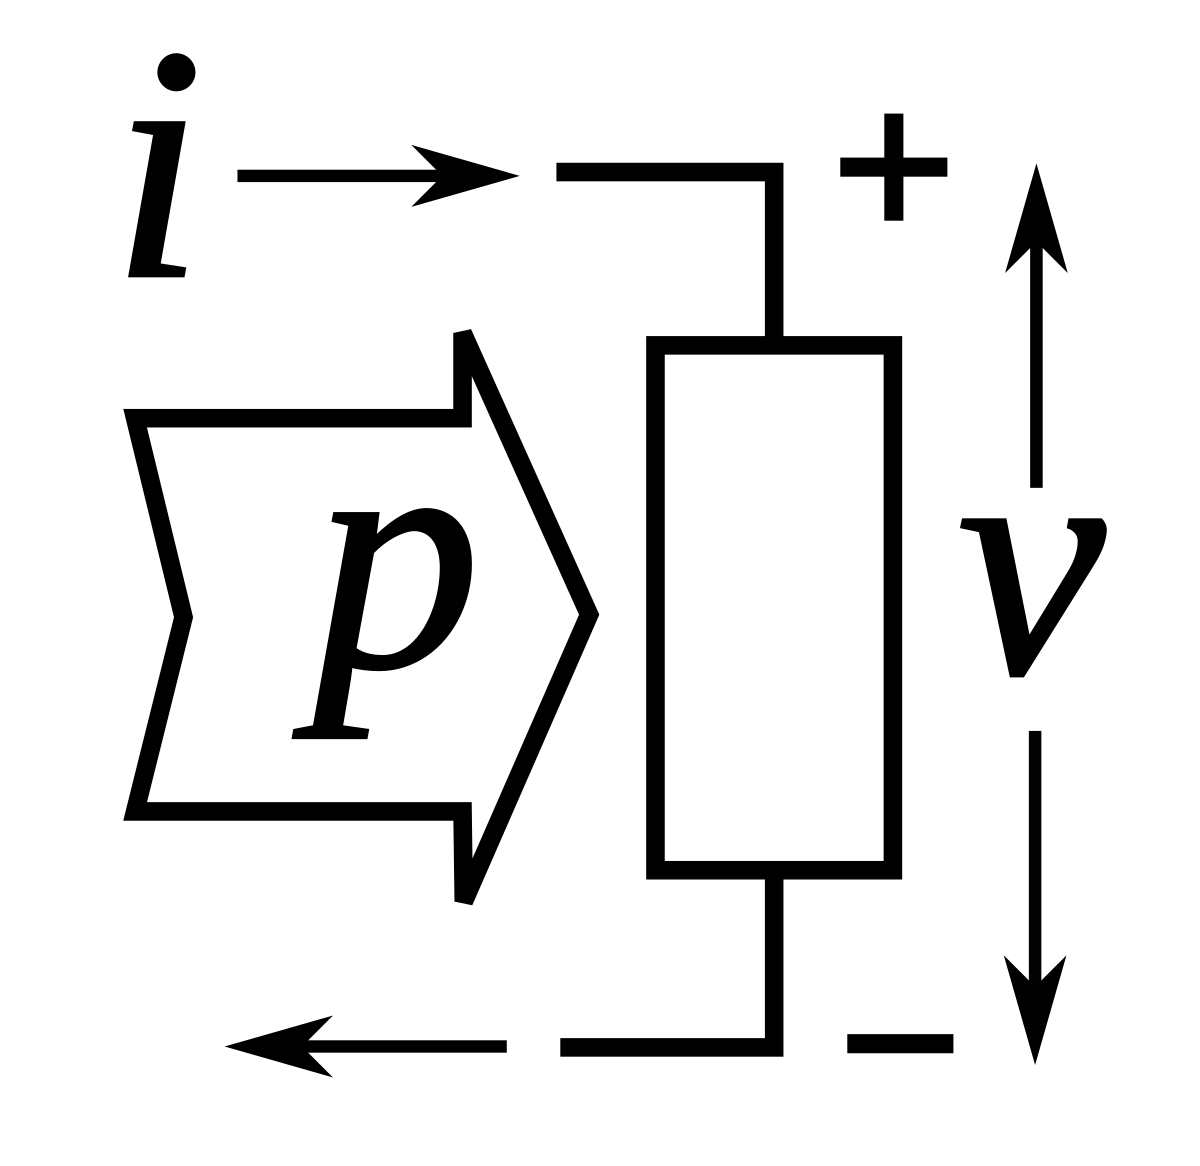
\includegraphics{images/Passive_sign_convention.svg.png}
    \caption{Passive sign convention}
    \label{fig:psc} 
\end{marginfigure}

\defn{Passive sign convention}{Defines current as going into 
positive terminal of component. The component loses energy 
and consumes power.
Defines electric power flowing out of the circuit into an electrical 
component as positive, and power flowing into the circuit out 
of a component as negative. So a passive component which 
consumes power, such as an appliance or light bulb, will 
have positive power dissipation, while an active component, 
a source of power such as an electric generator or battery, 
will have negative power dissipation.}

It's useful to have an idea of the components of circuit
schematics (visual representations of a circuit). Below is a list 
of the terms that will be used in this course:
\begin{itemize}
    \item Elements: The term elements means "components and sources."
    \item Symbols: Elements are represented in schematics by symbols. 
    Symbols for common 2-terminal elements are displayed to the right.
    
\begin{marginfigure}
    \centering
    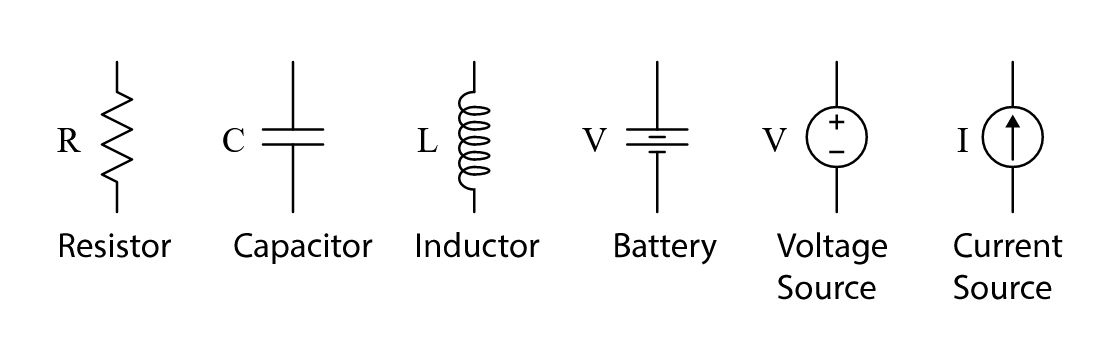
\includegraphics{images/symbols.png}
    \caption{Common circuit symbols}
    \label{fig:symbols}
\end{marginfigure} 

    \item Lines: Connections between elements are drawn as lines, 
    which we often think of as "wires". On a schematic, 
    these lines represent perfect conductors with zero resistance. 
    Every component or source terminal touched by a line is at the same voltage.
    \item Dots: Connections between lines can be indicated by dots. 
    Dots are an unambiguous indication that lines are connected. 
    If the connection is obvious, you don't have to use a dot.
\end{itemize}
Check out the circuit schematic below and see how many components you 
can identify!
\begin{center}
    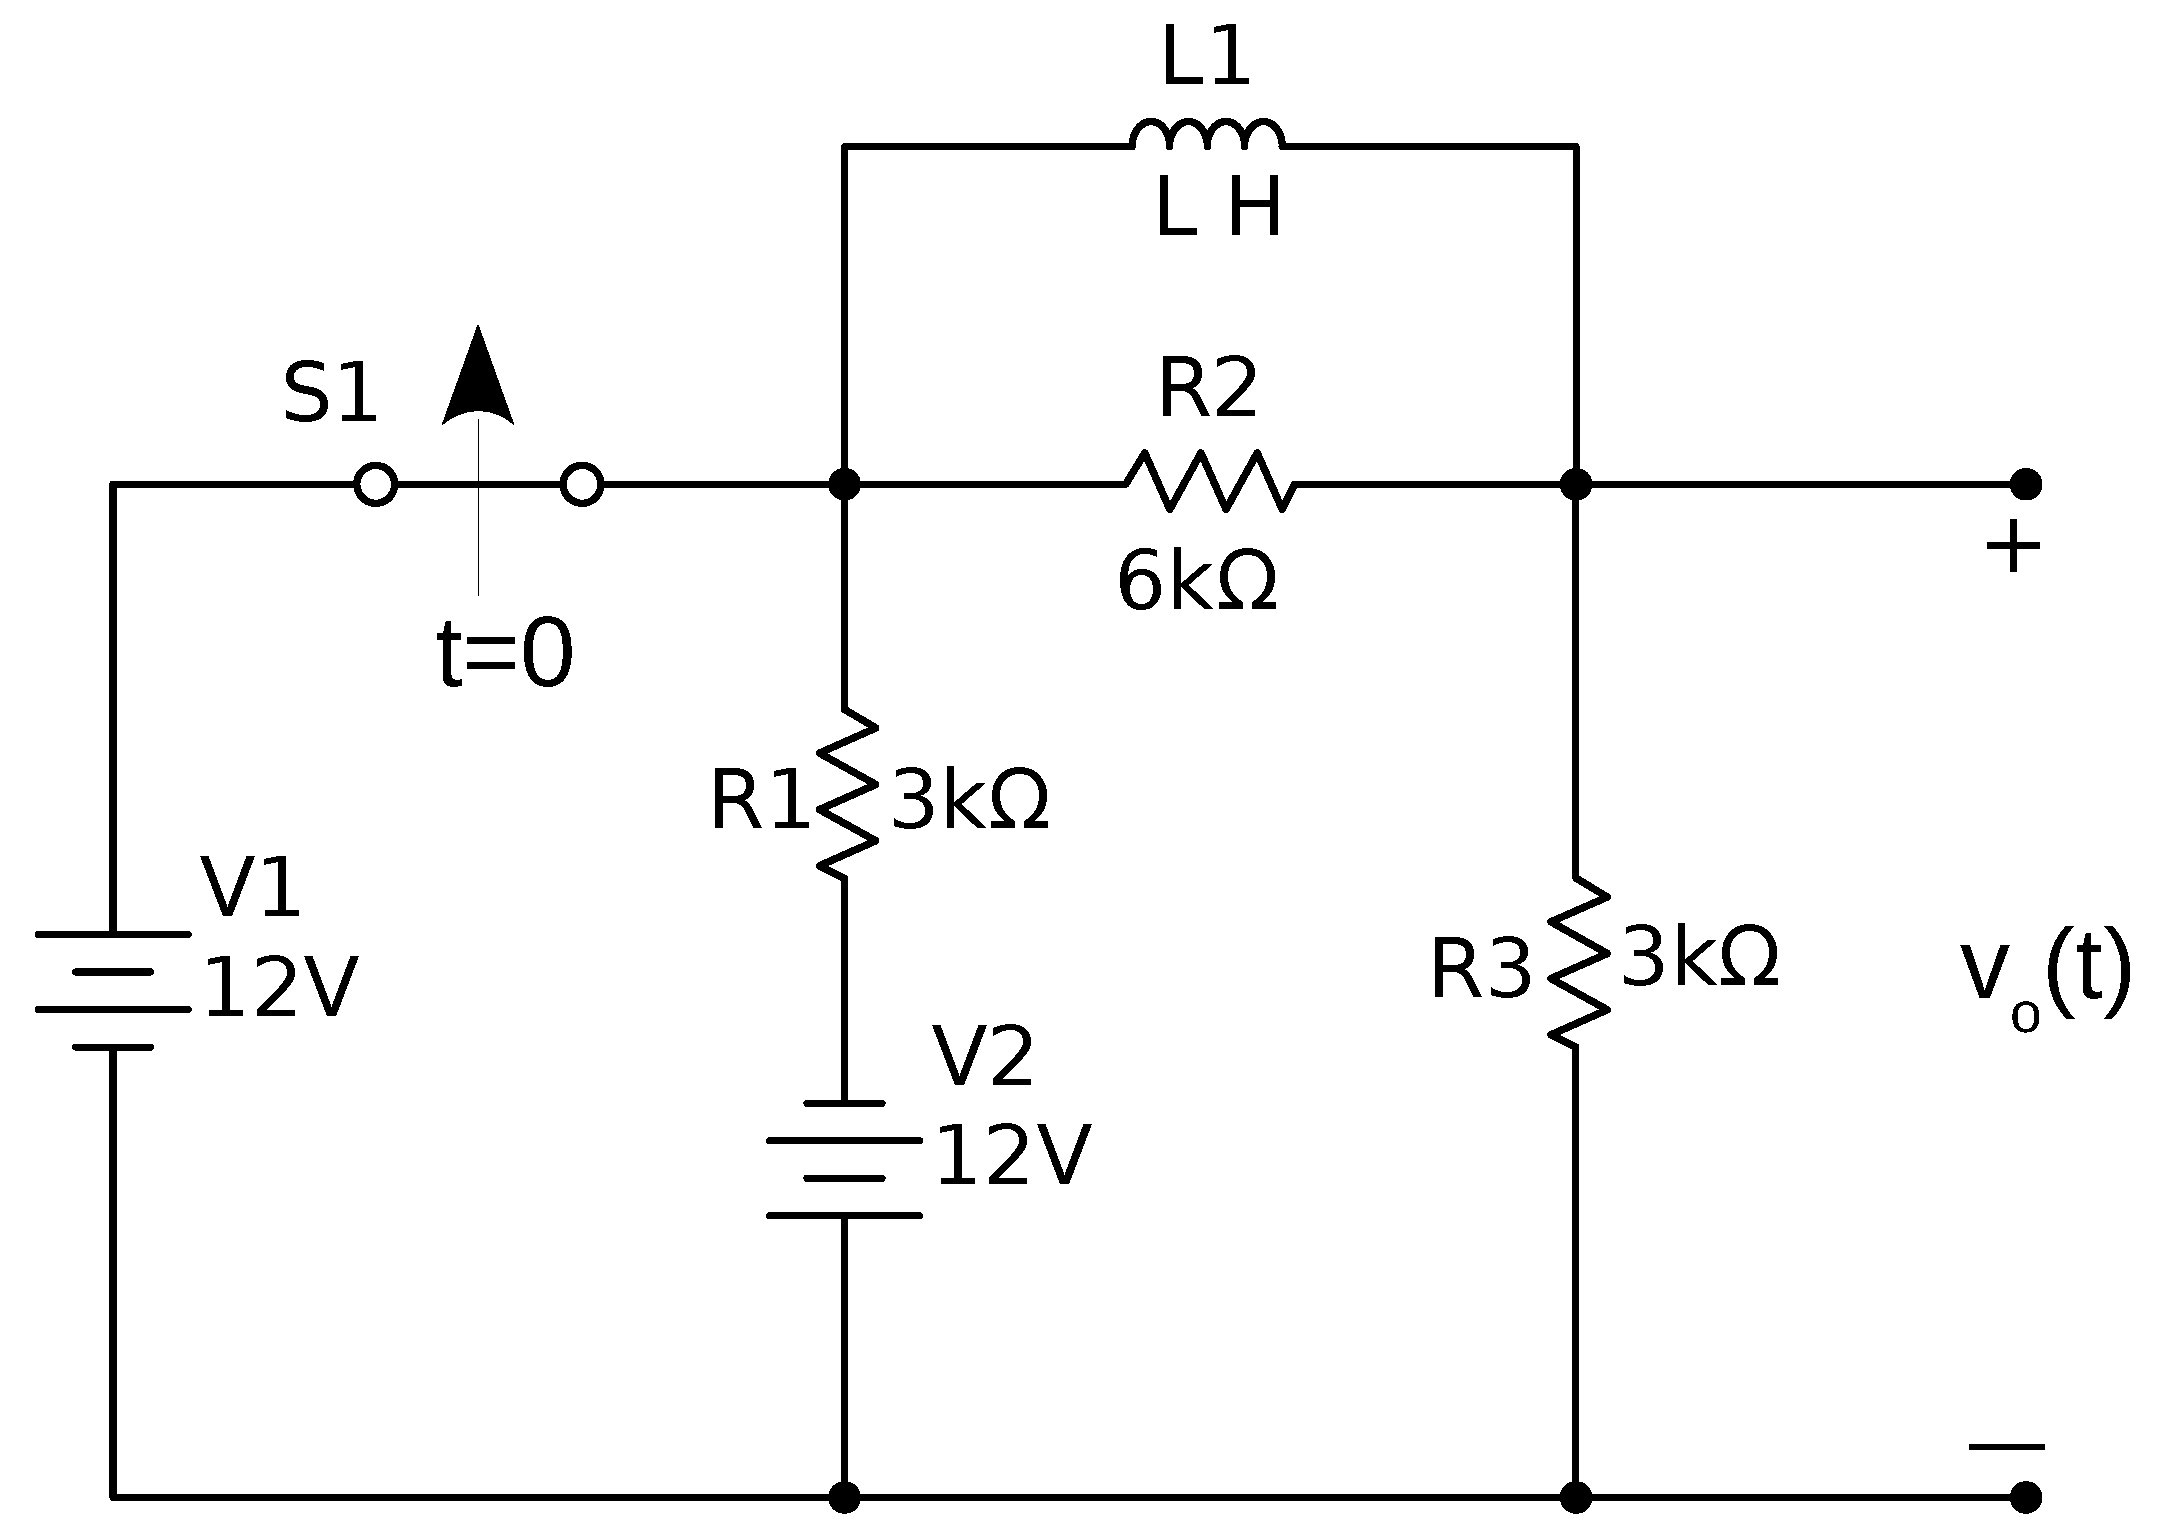
\includegraphics[width=\textwidth/2]{images/PS0_CapacitorCircuit.png}
\end{center}

Now, on to what circuits are doing. For interesting things
to happen we need electrons flowing through those wires.
Current is how quickly
electrons are moving along, or in more formal terms the rate of
change of charge. That is, $I = \frac{dQ}{dt}$. Its units are amperes (amps)
Voltage (or electric potential) is the amount of work done in moving charged 
particles such as electrons between two points. Whenever we want to separate 
two oppositely (positive and negative) charged particles or push two similarly-charged
particles together, we need to do
work to overcome the force between them. The work done in 
separating them is stored as potential energy.
This stored energy is known as electric potential (or voltage) and is measured in volts.
Thus, $V = \frac{W}{q}$. Just as with potential energy, voltage is always 
measured as a difference between two points. Power is the rate at which work is being done,
i.e. $P = \frac{dW}{dt}$. This would give power units of J/s, which
is known as Watts. Now, by rearranging the equation for voltage, we obtain also
$P=iV$. To make sense of this equation consider a light bulb in a circuit, with an electric potential difference of
5 V and a current flowing through of 10 A. The power used by the light bulb is 
$P=iV = 5 * 10 = 50$ watts, meaning it uses 50 J per second. 

\section{(In)dependent sources, connections, resistance and Ohm's Law}
Independent and dependent sources are fundamental elements in 
electrical circuits that provide voltage or current. 
They are used to model various types of input signals, 
power supplies, and components within a circuit.
Independent sources are voltage sources or current sources 
that maintain a constant value regardless of the rest of the 
circuit. They are not influenced by the circuit's current or 
voltage conditions. There are two main types of independent 
sources:
\begin{itemize}
    \item \defn{Independent voltage source}{Maintains a constant 
    voltage across its terminals, regardless of the current 
    flowing through it. It is typically represented by a 
    symbol with a plus sign and a minus sign, indicating 
    the polarity of the voltage.} A battery maintaining a constant
    voltage of 9 V is an example of an independent voltage source.
    \item \defn{Independent current source}{Maintains a constant 
    current through its terminals, regardless of the 
    voltage across it. It is usually represented by 
    a symbol with an arrow indicating the 
    direction of current flow.} Consider a current source that 
    provides a constant current of 2 amperes. This source 
    will deliver a current of 2A through any component 
    connected to it, regardless of the 
    voltage across the component.
\end{itemize}
Contrasted with independent sources, there are also
dependent sources. Dependent sources are sources 
whose values are 
dependent on other variables within the circuit. 
These sources are used to model components whose 
behavior changes according to the conditions in 
the circuit. There are four types of dependent sources:
\begin{itemize}
    \item \defn{Voltage-Controlled Voltage Source (VCVS)}{
    This type of dependent source generates a voltage 
    that is proportional to the voltage across a 
    separate part of the circuit. It is represented 
    as an ideal voltage source with a gain factor 
    that indicates the voltage ratio.}

    \item \defn{Current-Controlled Current Source (CCCS)}{
    This type of dependent source generates a current 
    that is proportional to the current flowing 
    through a different part of the circuit. It 
    is represented as an ideal current source with 
    a gain factor that indicates the current ratio.}

    \item \defn{Voltage-Controlled Current Source (VCCS)}{
    This type of dependent source generates a 
    current that is proportional to the 
    voltage across a different part of the 
    circuit. It is represented as an ideal 
    current source with a gain factor.}

    \item \defn{Current-Controlled Voltage Source (CCVS)}{
    This type of dependent source generates a 
    voltage that is proportional to the 
    current flowing through a separate part 
    of the circuit. It is represented as an 
    ideal voltage source with a gain factor.}
\end{itemize}

\defn{Series Combination}{In a series combination, the elements 
are connected with end to end in contact, such that 
current flow is equal in all the elements in the 
combination}

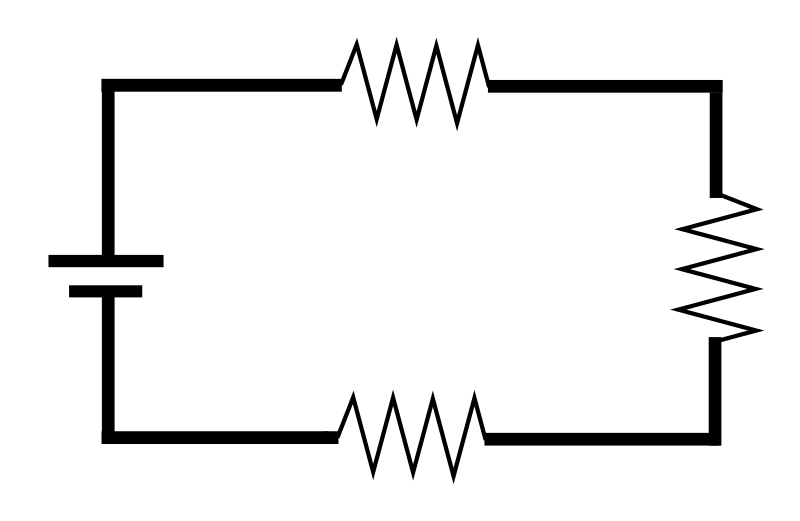
\includegraphics[width=\textwidth/2]{images/Series_circuit.svg.png}

\defn{Parallel Combination}{When two or more resistances are 
connected between the same two points, they are said to be 
connected in parallel combination. In this case voltage is equal
across all elements}

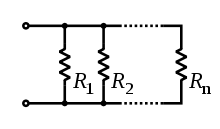
\includegraphics[width=\textwidth/2]{images/220px-Resistors_in_parallel.svg.png}

Turning off a voltage source is equivalent to replacing it with a 
short circuit (line). Turning off a current source is equivalent to replacing it with an
open circuit (broken line). Also equivalent to an open
circuit is a resistor with infinite resistance. 
Resistance is a measure of how hard it is to shove current
through a resistor. The harder it is, the higher the
resistance. It's given by $R = \frac{\rho L}{A} = \frac{V}{I}$, where $\rho$ 
is the resistivity, $L$ is the length of the resistor, and $A$ is the 
cross-sectional area of the resistor. The reciprocal of
resistance is conductance ($G = \frac{1}{R}$).

\end{document}
